Recurrent Neural Network (RNN) là một mạng neural hồi quy sử dụng dữ liệu tuần tự hoặc chuỗi thời gian với 3 thành phần chính là Input layer, Hidden layer và Output layer\cite{website2}.

Điểm đặc trưng của RNN là "bộ nhớ" của chúng cho phép sử dụng các thông tin từ đầu vào trước đó để ảnh hưởng đến đầu vào và đầu ra hiện tại, khác với mạng nơ-ron truyền thống.

Trong bài toán dự đoán giá vàng, RNN sử dụng 2 lớp SimpleRNN và Dense với từng vai trò khác nhau. Lớp SimpleRNN có tác dụng trích xuất các đặc trưng của dữ liệu chuỗi thời gian để nhận diện và học các bước xu hướng thời gian trước đó. Trong khi đó lớp Dense nhận các trích xuất đặc trưng từ lớp SimpleRNN và tổng hợp thông tin tin từ các đơn vị trong lớp RNN để áp dụng các phép biến đổi tuyến tính hoặc phi tuyến. Từ đó, dưới sự kết hợp của 2 lớp, mô hình RNN có thể đưa ra dự đoán giá vàng trong tương lai một cách chính xác.
\begin{figure}[htbp]
\centerline{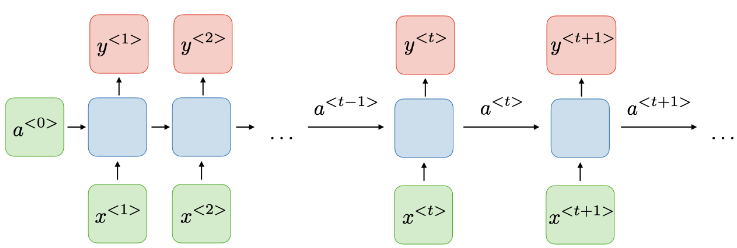
\includegraphics[width=0.4\textwidth]{img/RNN.png}}
\caption{Kiến trúc RNN}
\label{fig}
\end{figure}

RNN được biểu diễn bằng công thức sau:
\begin{align}
    a^{<t>} &= g_1(W_{aa}a^{<t-1>} + W_{ax}x^{<t>} + b_a) \\
    y^{<t>} &= g_2(W_{ya}a^{<t>} + b_y)
\end{align}

Trong đó:
\begin{itemize}
    \item $x^{<t>}$: giá trị đầu vào tại thời điểm $t$
    \item $y^{<t>}$: giá trị đầu ra tại thời điểm $t$
    \item $a^{<t>}$: giá trị kích hoạt
    \item $W_{aa}, W_{ax}, W_{ya}$: các ma trận trọng số
    \item $b_a, b_y$: vector độ lệch
    \item $g_1, g_2$: các hàm kích hoạt
\end{itemize}